\documentclass[12pt,a4paper]{article}
\usepackage[utf8]{inputenc}
\usepackage[english,russian]{babel}
\usepackage{amssymb,amsfonts,amsmath,cite,enumerate,float,indentfirst}
\usepackage{graphicx}
\usepackage{geometry}
\usepackage{systeme}
\usepackage{hyperref}
\usepackage{url}
\usepackage[bottom]{footmisc}
\hypersetup{
	colorlinks,
	citecolor=black,
	filecolor=black,
	linkcolor=black,
	urlcolor=black
}
\geometry{left=2cm}
\geometry{right=1.5cm}
\geometry{top=2cm}
\geometry{bottom=2cm}

\begin{document}
	
\begin{titlepage}
	\begin{center}		
		\vfill	
		Санкт-Петербургский политехнический университет \\
		Петра Великого\\
		\vskip 1cm
		Институт прикладной математики и механики \\
		Кафедра «Прикладная математика»
		\vfill
		\textbf{Отчёт\\
			по лабораторной работе №3\\
			по дисциплине\\
			«Математическая статистика»\\}
		\vfill
	\end{center}
	\vfill
	\hfill
	\begin{minipage}{0.4\textwidth}
		Выполнил студент:\\
		Самутичев Евгений Романович\\
		группа: 3630102/70201\\
	\end{minipage}
	\vfill
	\hfill 
	\begin{minipage}{0.4\textwidth}
		Проверил:\\
		к.ф.-м.н., доцент\\
		Баженов Александр Николаевич\
	\end{minipage}
	\vfill
	\begin{center}
		Санкт-Петербург\\2020 г.
	\end{center}
\end{titlepage}

\tableofcontents
\listoffigures
\listoftables
\pagebreak

\section{Постановка задачи}
Для каждого из 5 распределений:

\begin{enumerate}
	\item Нормального $N(x, 0, 1)$
	\item Коши $C(x, 0, 1)$
	\item Лапласа $L(x, 0, \frac{1}{\sqrt{2}})$
	\item Пуассона $P(k, 10)$
	\item Равномерного $U(x, -\sqrt{3}, \sqrt{3})$	
\end{enumerate}

сгенерировать выборки размера 20 и 100, построить боксплот Тьюки. Определить долю выбросов экспериментально (сгенерировав выборку каждого размера 1000 раз) и сравнить с результатами полученными теоретически.
\pagebreak

\section{Теория}
\subsection{Выбросы}
\subsubsection{Определение}
Результат измерения, выделяющийся из выборки называется \textit{выбросом}. Простейший критерий основан на межквартильном расстоянии, выбросами считаются элементы выборки лежащие вне диапазона $[X_1, X_2]$:
\begin{equation}\label{1}
X_1=LQ - \frac{3}{2}(UQ-LQ), X_2=UQ + \frac{3}{2}(UQ-LQ)
\end{equation}, где $LQ, UQ$ - выборочные нижний и верхний квартили.

Теоретическая вероятность выбросов для непрерывных распределений:
\begin{equation}\label{2}
P_{outlier} = P(x<X_1) + P(x>X_2) = F(X_1) + (1 - F(X_2))
\end{equation}
, а для дискретных с учетом возможного скачка
\begin{equation}\label{3}
P_{outlier} = F(X_1) - (F(X_1+) - F(X_1)) + (1 - F(X_2))
\end{equation}

\subsubsection{Доля выбросов}
Проведем следующий эксперимент $1,...,i,...,N$ раз: сгенерируем выборку размера $n$ и подсчитаем число выбросов $k_i$, используя определение \hyperref[1]{(1)}, но с выборочными квартилями. Тогда доля выбросов в $i$-м эксперименте:
\begin{equation}
	P_i = \frac{k_i}{n}
\end{equation}

Собственно \textit{долей выбросов} будем называть величину
\begin{equation}\label{5}
	P = \frac{1}{N}\sum_{i=1}^{N} P_i
\end{equation},
с дисперсией
\begin{equation}\label{6}
	D = \frac{1}{N}\sum_{i=1}^{N} P_i^2 - P^2
\end{equation}

\subsection{Боксплот Тьюки}
\subsubsection{Описание}
\textit{Боксплот} (англ. box plot) — график, использующийся в описательной статистике, компактно изображающий одномерное распределение вероятностей: в удобной форме показывает медиану, нижний и верхний квартили, минимальное и максимальное значение выборки и выбросы.\cite{boxplot}

\subsubsection{Построение}
Границами ящика служат $LQ \text{ и } UQ$, линия в середине ящика — медиана. Концы усов — края статистически значимой выборки (без выбросов): $X_1 \text{ и } X_2 \text{ }\hyperref[1]{(1)}$.

\pagebreak

\section{Реализация}
\label{sec:impl}
Работа выполнена с использованием языка \textbf{Python} в интегрированной среде разработки \textbf{PyCharm}, были задействованы библиотеки:

\begin{itemize}
	\item \textbf{NumPy} - вычисление квартилей для дальнейшего подсчета выбросов
	\item \textbf{SciPy} - модуль \textbf{stats} для генерации данных по распределениям
	\item \textbf{Matplotlib} - построение боксплотов
\end{itemize}

Исходный код работы приведен в приложении. 
\pagebreak

\section{Результаты}
\subsection{Боксплоты}
\begin{figure}[h!]
	\centering
	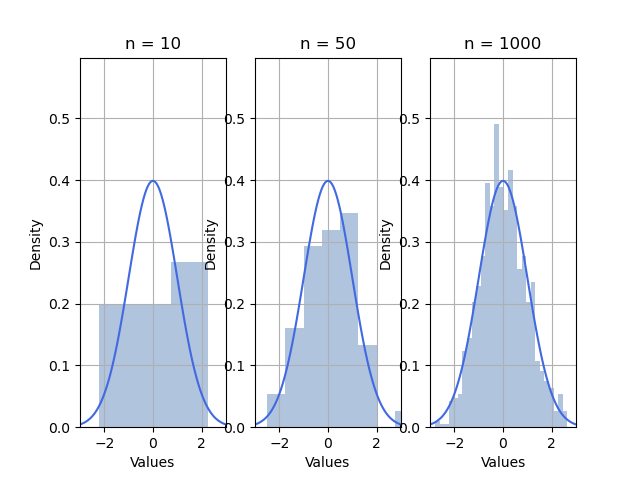
\includegraphics[scale=0.8]{normal.png}
	\caption{Нормальное распределение}
	\label{fig:image}
\end{figure}

\begin{figure}[h!]\label{4}
	\centering
	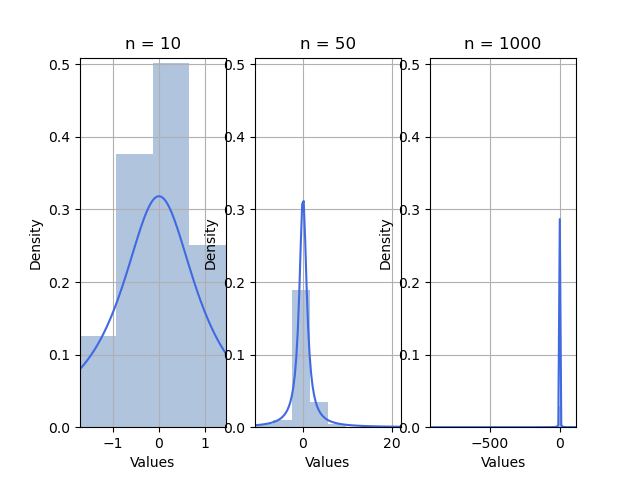
\includegraphics[scale=0.8]{cauchy.png}
	\caption{Распределение Коши}
	\label{fig:image:cauchy}
\end{figure}

\pagebreak

\begin{figure}[h!]
	\centering
	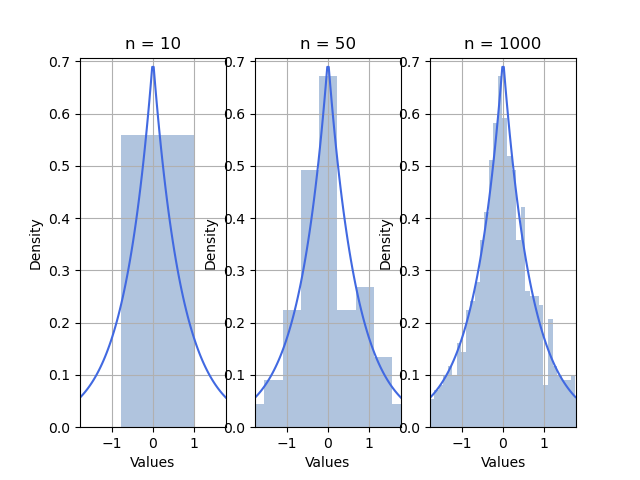
\includegraphics[scale=0.8]{laplace.png}
	\caption{Распределение Лапласа}
	\label{fig:image}
\end{figure}

\begin{figure}[h!]
	\centering
	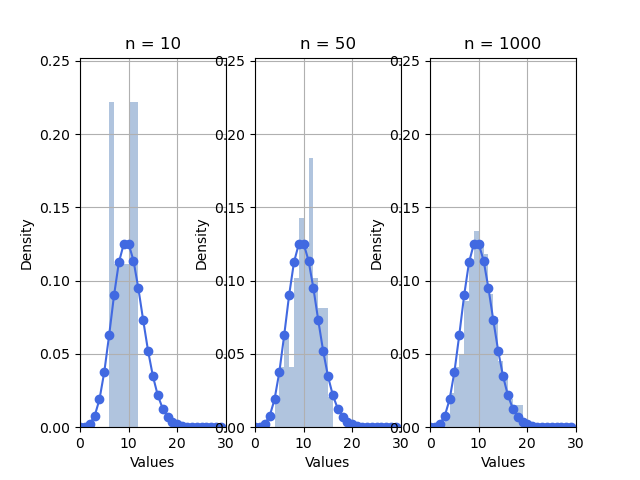
\includegraphics[scale=0.8]{poisson.png}
	\caption{Распределение Пуассона}
	\label{fig:image}
\end{figure}

\pagebreak

\begin{figure}[h!]
	\centering
	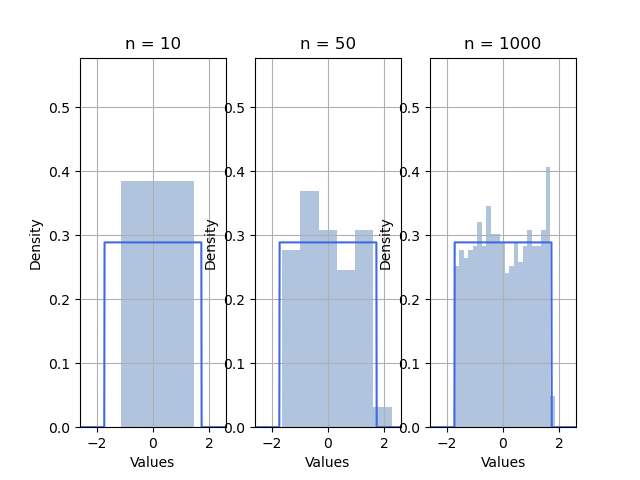
\includegraphics[scale=0.8]{uniform.png}
	\caption{Равномерное распределение}
	\label{fig:image}
\end{figure}
\pagebreak

\subsection{Теоретическая вероятность выбросов}
Подсчитана для каждого распределения при помощи модуля {stats} библиотеки {SciPy} (см. \hyperref[sec:impl]{Реализация}):

\begin{table}[h!]
	\centering
	\begin{tabular}{|l|l|l|l|l|l|}
		\hline
		Распределение&normal&cauchy&laplace&poisson&uniform  \\ \hline
		$P_{outlier}\text{	} \hyperref[2]{(2)},\hyperref[3]{(3)}$
		&0.007  &0.156  &0.0625  &0.008  &0.0  \\ \hline
	\end{tabular}
	\caption{Теоретическая вероятность выбросов}
\end{table}

\subsection{Доля выбросов}
\begin{table}[h!]
	\centering
	\begin{tabular}{|l|l|l|l|l|l|}
		\hline
		Распределение&normal&cauchy&laplace&poisson&uniform  \\ \hline
		$n=20$& & & & & \\ \hline
		$P\hyperref[5]{(5)}$&0.025 &0.147 &0.070 &0.022 &0.0023  \\ \hline
		$D\hyperref[6]{(6)}$&0.002085 &0.005248 &0.004219 &0.001801 &0.0002  \\ \hline
		$n=100$& & & & & \\ \hline
		$P$&0.0105 &0.156 &0.0658 &0.0108 &0.0  \\ \hline
		$D$&0.000185 &0.001068 &0.0009 &0.000236 &0.0 \\ \hline
	\end{tabular}
	\caption{Доля выбросов}
\end{table}

\pagebreak

\section{Обсуждение}
Из полученных таблиц видно что доля выбросов близка к теоретической. Наибольшая при этом у распределения Коши, что также видно по боксплоту Тьюки \hyperref[fig:image:cauchy]{(рис. 2)}. Вторая по величине у распределения Лапласа. Для остальных выборок доля выбросов не превосходит $95\%$, а значит можно считать что они соответствуют гипотетическим распределениям.

\pagebreak

\section{Приложения}
\noindent 1. Исходный код лабораторной {\url{https://github.com/zhenyatos/statlabs/tree/master/Lab3}}

\begin{thebibliography}{9} 
	\bibitem{chernova} Н. И. Чернова, \emph{Математическая статистика: Учеб. пособие}. Новосиб. гос. ун-т. Новосибирск, 2007. 148 стр.
	\bibitem{boxplot} Ящик с усами // Википедия. [2020—2020]. Дата обновления: 12.01.2020. URL: \url{https://ru.wikipedia.org/?oldid=104502300} (дата обращения: 12.01.2020)
\end{thebibliography}

\end{document}
